%!TEX root = ../report.tex

% 
% Introduction
% 

\section{Introduction}

%General description of the problem and its context, current solutions, and road map of the project.

%This days designers and developers have available a large number of Computer Aided Design(CAD) tools to produce their models. This tools are getting more and more powerful and with more features available. The traditional way of modeling where the user adds geometry one by one does not present performance issues about rendering. On the other hand it is being more and more common the concept of generative design, that is a design method that is based on a programming approach which allows architects and designers to model large amounts of shapes with significantly less effort.

%As technology evolves people have more powerful devices and they want to take advantage of that. They want to have more realistic experiences with larger, more detailed and complex contents.
%And this is observable in the graphic contents. With the recent extra high definition on screens and the computational power of the machines beating records, the graphic content has to follow up that characteristics in quantity as well as in quality. The issue is that the manual content generation takes a long work time from architects and designers to achieve this quality, which implies high costs.

Graphic contents are mainly used for entertainment, both in the gaming and movie industries, but they are also used in many other different areas. The fields of architecture and design, for instance, use this technology to experiment and model new designs, from small objects like a plate, to buildings or even entire cities. Unfortunately, manual modeling of large sets of potentially complex shapes is tiresome and very costly. 
%In this field they also face the problems that raises from the modeling of really big sets of objects and forms manually, which is slow and error prone. \emph{This work addresses the problem of large content creation and will focus on the fields of architecture and design.}
The obvious solution to this problem is to hire more architects or designers in order to increase productivity and reduce the time needed. However, experience has shown that this solution is not scalable, because doubling the number of architects or designers working in a project will not double their overall productivity. Also, this solution has a big impact on financial costs, that would take immediately out of the market producers with fewer resources.

A solution for this problem is the use of generative design (GD). This is a design method that is based on a programming approach which allows architects and designers to model large volumes of complex shapes with significantly less effort. They can model cities, buildings, trees, and many other objects that are, usually, too big or complex for a manual approach.


\begin{wrapfigure}{r}{0.5\textwidth}
%	\vspace{-15pt}
    \centering
	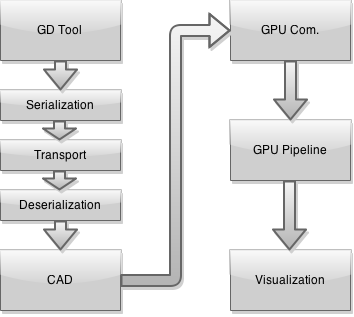
\includegraphics[width=0.5\textwidth]{img/Architecture/GD-Common-Pipeline.png}
	\caption{Common Generative Design Pipeline}
	\label{fig:GD_Pipeline}
	\vspace{-15pt}
\end{wrapfigure}


Although most computer-aided design (CAD) applications provide programming languages for generative design, programs written in these languages have very limited portability. Additionally, the provided languages, such as AutoLisp, C++ or Visual Basic, are not pedagogical and are difficult to use even to experienced programmers. All this problems create barriers to the adherence to this approach by all users, specially those that are not used to code.\cite{ramos_et_al:OASIcs:2014:4565}

There are several generative design (GD) tools such as Grasshopper\footnote{\url{http://www.grasshopper3d.com/}} and Rosetta\cite{Leit2012}, that aim to break down some of this barriers, and facilitate the approximation of these individuals to programming. With this tools the users can create their models using pedagogical and easy to use languages. This systems implement a straightforward pipeline presented in Figure~\ref{fig:GD_Pipeline}.


%\begin{figure}[htbp]
%	\centering
%	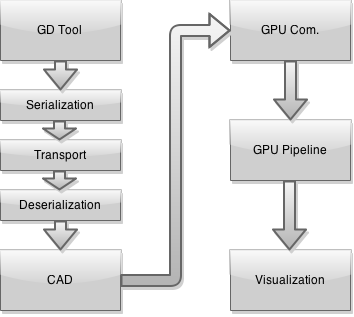
\includegraphics[width=0.45\textwidth]{img/Architecture/GD-Common-Pipeline.png}
%	\caption{Common Generative Design Pipeline}
%	\label{fig:GD_Pipeline}
%\end{figure}

Architects and designers implement their models on GD tools. Users implement their models through the GD tool interface. Then all the geometry data is serialized and the data is transfered through some transport mechanism. This data has to be deserialized on the other side within the CAD application. The CAD application takes the deserializes data and processes it producing geometry. Finally, the geometry is moved to the GPU that renders it. All these steps are time-consuming, due to the large amount of data that needs to be transfered. This creates a performance problem.

One big difference between GD and traditional approaches is that users do not see the result of their program while they code. They follow a code-execute-visualize loop where they make changes in the code, execute the code and visualize the resulting model. This makes it difficult for them to understand the impact of changes in their programs. It would be much more productive if they could easily understand the correlation between their program and the resulting model and to be able to experiment values on their program and see the effects they have on the model. To help them with this, there is the concept of \emph{immediate feedback}. Immediate feedback is a mechanism that allows the users to quickly see the results of the changes they make. This can be implemented, for instance, through the use of sliders that can be associated with values on the program, and when one slider is moved the effects of that change should be visualized immediately. 

However, there is a problem: CAD applications are built for manual modeling mainly, and are not prepared to quickly handle large amounts of geometry. Running the code produces much more geometry and much faster than manual modeling, so the user is able to create massive amounts of geometry, which is fed to the CAD that gets overloaded. With this issues, it is hard to get good performance, specially with large models, that makes impossible to have true immediate feedback, which mainly requires visualization, that is only one of the concerns of a CAD application. Because of that users sometimes have to wait long periods of time for the model to be rendered.

This work proposes a solution to this problem and aim to generate large volumes of geometry that is as close as possible to real-time. It does so by jumping over some steps while drastically decreasing the amount of data that is transfered between steps. First we aim to get the geometry as fast as possible to the GPU, so since our goal is just visualization, we jump the CAD layer, eliminating the first communication steps. Another action is to reduce the amount of data that is transferred, by transferring only a very concise description of the geometry, generating the actual geometry on the GPU. To implement the generation of the geometry, procedural techniques such as: Fractals(Section~\ref{ssub:fractals}), Cellular Automata (Section~\ref{sub:cellular_automaton}), and L-Systems (Section~\ref{ssub:l_systems}) will be applied. 
To improve performance with visualization, techniques such as Level Of Detail (Section~\ref{ssub:level_of_detail}) and Occlusion Culling (Section~\ref{ssub:occlusion_culling}) are explored.

